\chapter{Planificación}

Para abordar el problema discutido en la sección anterior y superar las limitaciones que presentan las soluciones actuales, se desarrollará \textbf{GAC} (Gestor Académico de Calendarios), una plataforma web innovadora diseñada para los estudiantes de la Universidad de Granada. Esta plataforma facilitará la gestión de sus horarios académicos de manera intuitiva, sencilla y eficiente. GAC no solo integrará las funcionalidades básicas de las soluciones ya existentes, sino que también las potenciará con una serie de características adicionales que harán la experiencia del usuario mucho más completa y personalizada. Dichas características incluyen:

\begin{enumerate} 
    \item \textbf{Centralización de la información:} GAC reunirá en un único lugar toda la información académica relevante para los estudiantes, como asignaturas, grupos y horarios. Esta centralización permitirá acceder de forma rápida y sencilla a todos los datos necesarios, evitando la dispersión de la información en diferentes plataformas o documentos.

    \item \textbf{Gestión de horarios optimizada:} La plataforma ofrecerá una gestión automática de horarios, buscando evitar solapamientos entre clases y garantizando la distribución más óptima de las asignaturas a lo largo de la semana. Los estudiantes podrán personalizar sus horarios según sus preferencias y necesidades, lo que les permitirá planificar su tiempo de manera más efectiva.

    \item \textbf{Exclusividad en el enfoque:} GAC se destacará por su enfoque exclusivo en la gestión de calendarios académicos, ofreciendo una solución especializada y adaptada a las necesidades específicas de los estudiantes universitarios. A diferencia de otras herramientas genéricas, GAC se centrará en proporcionar una experiencia más completa y adaptada a los usuarios, mejorando significativamente las funcionalidades ya disponibles y añadiendo nuevas características para un manejo más eficiente y personalizado. 
\end{enumerate}

Con estas mejoras, GAC se posicionará como una herramienta indispensable para los estudiantes de la Universidad de Granada, facilitando su organización académica y contribuyendo a un mejor aprovechamiento de su tiempo y recursos.

\section{Metodología de Desarrollo Ágil}

La ingeniería de software es una disciplina que ha evolucionado significativamente para adaptarse a los avances tecnológicos y a las necesidades cambiantes de las empresas modernas. Esto se ha logrado mediante la creación de métodos efectivos que guían el proceso hasta alcanzar el producto final de software. Uno de estos métodos exitosos es el desarrollo ágil de software. Este enfoque ágil es más ligero y fue diseñado para superar las limitaciones de los métodos de desarrollo más tradicionales y complejos, reduciendo así tanto el costo como la carga de trabajo. Al mismo tiempo, ofrece una gran flexibilidad para incorporar cambios en los requisitos en cualquier fase del proyecto, lo que se logra a través de una gestión y coordinación de tareas basada en un conjunto específico de valores y principios fundamentales \cite{AlSaqqa2020AgileSD}.\newline

Dichos valores y principios se encuentran recogidos en el Manifiesto Ágil \cite{beck2001agile}. Algunas de esas premisas son:

\begin{itemize}
    \item \textbf{Flexibilidad y adaptabilidad:} el desarrollo ágil se basa en la capacidad de adaptarse a los cambios y responder a ellos de manera efectiva.
    \item \textbf{Desarrollo iterativo e incremental:} el desarrollo ágil se basa en la creación de versiones del producto en ciclos cortos y regulares, lo que permite obtener retroalimentación temprana y realizar ajustes en función de ella.
    \item \textbf{Entregas continuas:} el desarrollo ágil se basa en la idea de que es mejor entregar un producto funcional en partes pequeñas y regulares que esperar a tener un producto completo.
    \item \textbf{Simplicidad:} el desarrollo ágil se basa en la idea de que la simplicidad es esencial para el éxito del proyecto. Se busca minimizar la complejidad y centrarse en lo esencial.
\end{itemize}

\subsection{Ejemplos de Metodologías Ágiles}

\begin{enumerate}
    \item \textbf{Kanban:} Se trata de un método visual para la gestión de proyectos que se basa en la utilización de tableros y tarjetas para representar las tareas y su estado. Kanban es una metodología ágil que se centra en la mejora continua y en la optimización del flujo de trabajo. En un tablero Kanban (Figura \ref{fig:kanban}), las tareas se dividen en columnas que representan diferentes estados del proceso, como "pendiente", "en progreso" y "completado". Los miembros del equipo pueden mover las tarjetas de una columna a otra a medida que avanzan en su trabajo, lo que permite visualizar de forma clara y sencilla el estado de las tareas y identificar posibles cuellos de botella o retrasos.
    \begin{figure}[H]
        \centering
        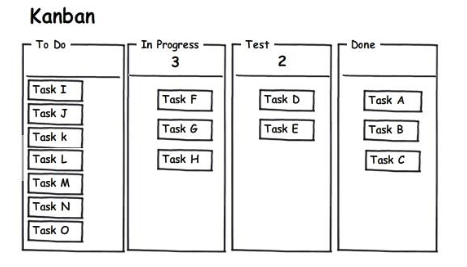
\includegraphics[width=0.7\textwidth]{imagenes/kanban.png}
        \caption{Ejemplo de tablero Kanban \cite{kirovska2015usage}.}
        \label{fig:kanban}
    \end{figure}
    \item \textbf{Scrum:} Es un marco de trabajo ágil que se centra en la colaboración, la transparencia y la adaptabilidad. En Scrum, los proyectos se dividen en iteraciones cortas llamadas ``sprints'' (Figura \ref{fig:scrum}), que suelen tener una duración de 2 a 4 semanas. Durante cada sprint, el equipo se compromete a completar un conjunto de tareas específicas y al final del sprint se realiza una revisión para evaluar los resultados y planificar el siguiente sprint. Scrum se basa en roles definidos, como el ``Product Owner'', el ``Scrum Master'' y el ``Equipo de Desarrollo'', que trabajan juntos para lograr los objetivos del proyecto.
    \begin{figure}[H]
        \centering
        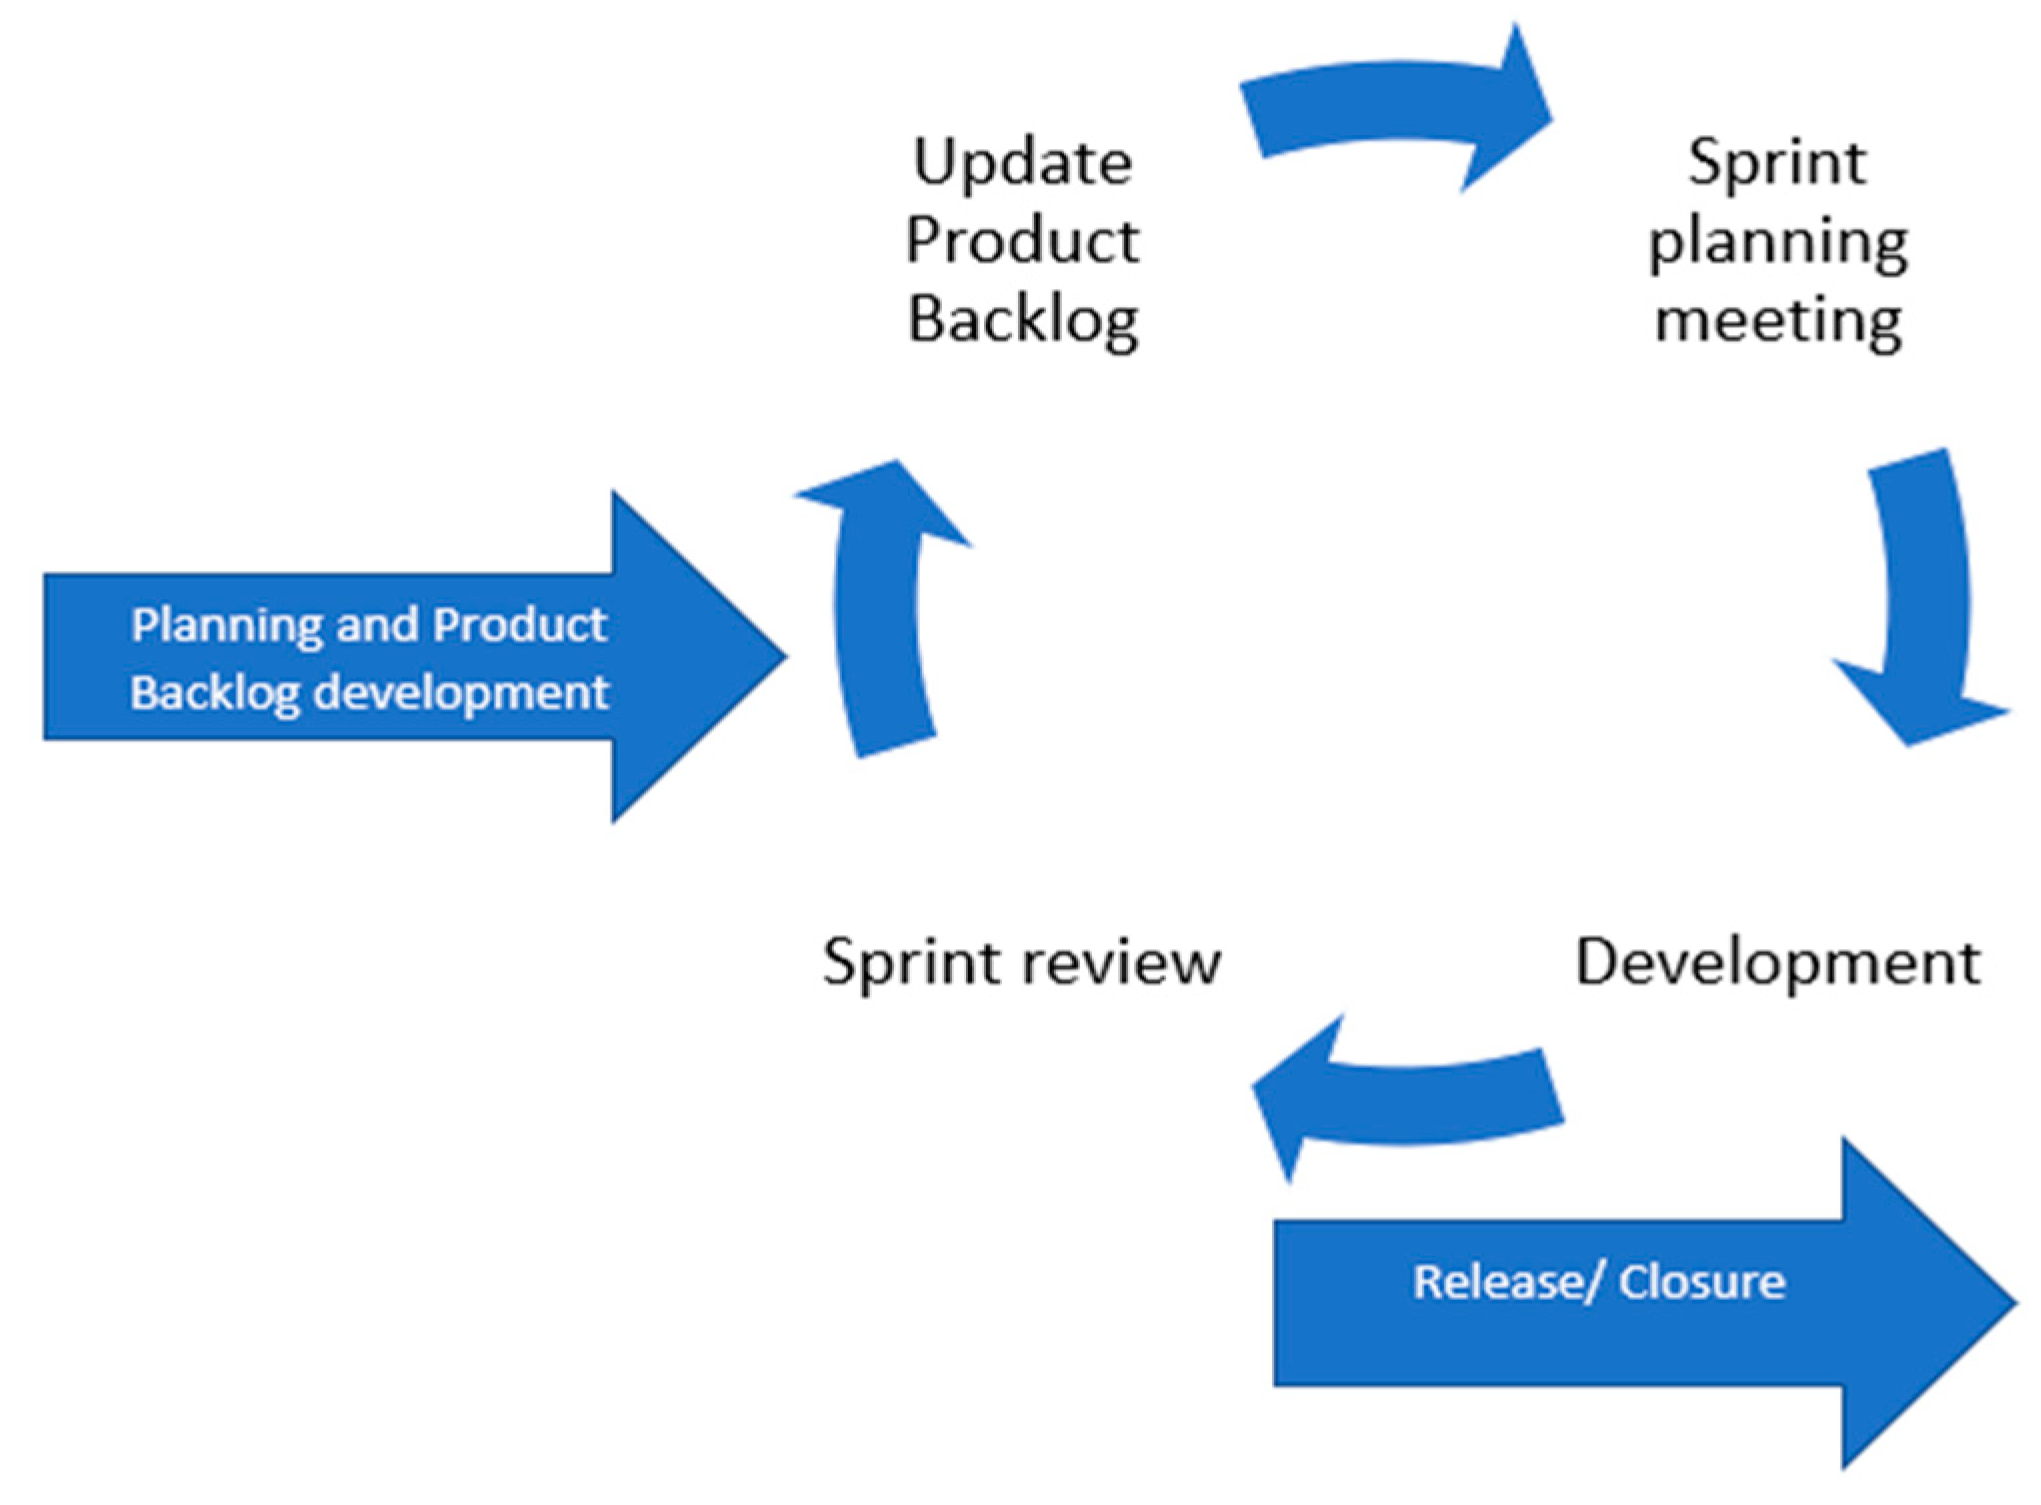
\includegraphics[width=0.7\textwidth]{imagenes/scrum.png}
        \caption{Ejemplo de tablero Scrum \cite{karabiyik2020understanding}.}
        \label{fig:scrum}
    \end{figure}
    \item \textbf{Lean:} Es una metodología ágil que se centra en la eliminación de desperdicios (Figura \ref{fig:lean}) y la maximización del valor para el cliente. Lean se basa en el concepto de ``valor'' y busca identificar y eliminar todo aquello que no aporta valor al cliente. Al eliminar los desperdicios y optimizar los procesos, Lean permite a las organizaciones ser más eficientes y competitivas.
    \begin{figure}[H]
        \centering
        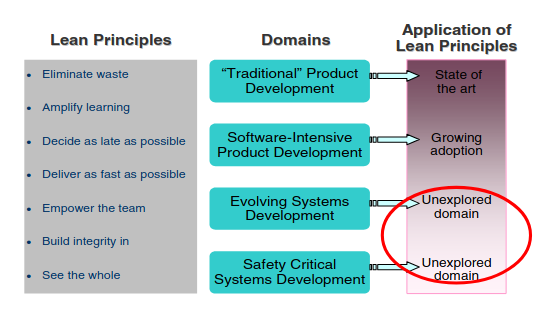
\includegraphics[width=0.7\textwidth]{imagenes/lean.png}
        \caption{Principios de Lean \cite{cawley2010lean}.}
        \label{fig:lean}
    \end{figure}
\end{enumerate}

Para llevar a cabo este proyecto, se ha optado por una metodología de desarrollo ágil, en este caso \textbf{Scrum}. Esta elección fue motivada por las siguientes razones:

\begin{enumerate}
    \item \textbf{Flexibilidad:} Al asumir los roles de programador y usuario de la aplicación, la capacidad de adaptación cobró gran relevancia. Los requisitos podían modificarse conforme progresaba el desarrollo. La implementación de Scrum, con sus ciclos de trabajo cortos (sprints) y revisiones frecuentes, me permitió ajustar el producto a medida que avanzaba el proyecto.
    \item \textbf{Desarrollo incremental:} Scrum se basa en la idea de que es mejor entregar un producto funcional en partes pequeñas y regulares que esperar a tener un producto completo. Esta filosofía me permitió avanzar en el desarrollo de la plataforma de manera progresiva y constante, entregando funcionalidades completas y probadas en cada sprint.
    \item \textbf{Iteratividad:} La metodología Scrum se basa en la creación de versiones del producto en ciclos cortos y regulares. Esto me permitió obtener retroalimentación temprana y realizar ajustes en función de ella, lo que resultó fundamental para el éxito del proyecto.
\end{enumerate}

\section{Temporización}

El proyecto comenzó en Diciembre de 2023. Para ilustrar la planificación del proyecto, se utiliza un Diagrama de Gantt. Este tipo de diagrama es una representación gráfica del cronograma del proyecto (Figura \ref{fig:cronograma}). El Diagrama de Gantt permite visualizar claramente las fechas de inicio y finalización de cada tarea, lo que facilita el seguimiento del progreso y la gestión eficiente de las diferentes etapas del desarrollo.

\begin{figure}[H]
    \centering
    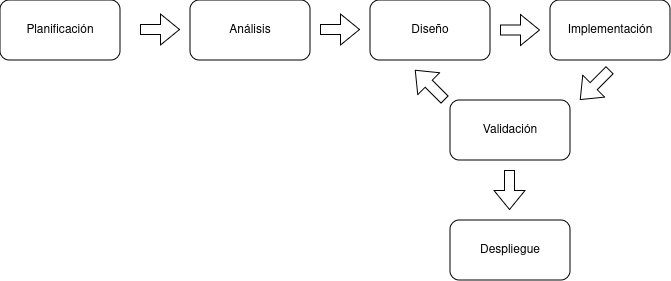
\includegraphics[width=1\textwidth]{imagenes/cronograma.png}
    \caption{Cronograma del proyecto.}
    \label{fig:cronograma}
\end{figure}

\subsection{Diagrama de Gantt}

El desarrollo completo de la plataforma se ha extendido a lo largo de 8 meses. Durante este período, se llevaron a cabo las diversas etapas del proyecto, las cuales se detallan en el siguiente diagrama de Gantt (Figura \ref{fig:gantt}).

\begin{figure}[H]
    \centering
    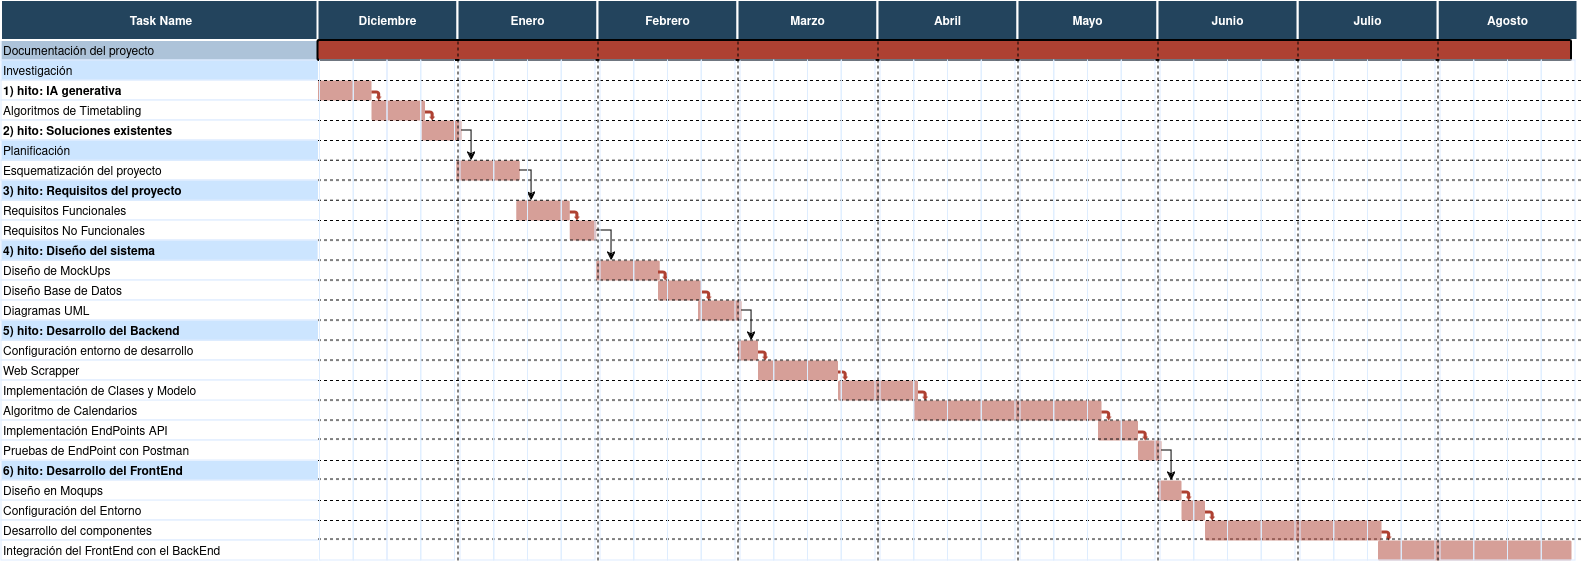
\includegraphics[width=1\textwidth]{imagenes/gantt.png}
    \caption{Diagrama de Gantt del proyecto.}
    \label{fig:gantt}
\end{figure}

\section{Recursos y costes}

En este apartado se discuten los recursos y materiales empleados en el desarrollo del proyecto, así como los costes asociados a los mismos.

\subsection{Recursos humanos}

Para el desarrollo de la plataforma \textbf{GAC}, se ha contado con un único desarrollador, el autor de este documento. Además, cabe destacar la labor de mis tutores, quienes han supervisado y guiado el desarrollo del mismo.

\subsection{Materiales}

Para el desarrollo de la plataforma se ha utilizado un portátil personal y un segundo monitor (Figura \ref{tab:coste_materiales}), el cual ha sido de gran utilidad para la realización de tareas de desarrollo y diseño, al permitir visualizar de forma simultánea varias ventanas y herramientas. Ambos dispositivos son propiedad del autor.

% Please add the following required packages to your document preamble:
% \usepackage{multirow}
\begin{table}[H]
    \begin{tabular}{|c|c|c|ll}
    \cline{1-3}
    \multicolumn{1}{|l|}{Concepto}                                                                              & \multicolumn{1}{l|}{Coste Unitario (€)} & \multicolumn{1}{l|}{Coste Materiales (€)} &  &  \\ \cline{1-3}
    \begin{tabular}[c]{@{}c@{}}Acer Aspire 3 A315-59-504M -\\  Intel® Core™ i5-1235U -\\  16GB RAM\end{tabular} & 749 €                                   & \multirow{2}{*}{846,90€}                  &  &  \\ \cline{1-2}
    \begin{tabular}[c]{@{}c@{}}Monitor -\\ Asus VZ239HE 23" Full HD IPS\end{tabular}                            & 97,90€                                  &                                           &  &  \\ \cline{1-3}
    \end{tabular}
    \caption{Coste de Materiales}
    \label{tab:coste_materiales}
\end{table}


\subsection{Presupuesto}

En esta sección se examinan y detallan los costos del proyecto. Se considerará el perfil de un ingeniero informático Junior, tomando en cuenta que el salario anual oscila entre los 20.000 € - 28.000 € \footnote{\url{https://www.glassdoor.es/Sueldos/junior-software-engineer-sueldo-SRCH_KO0,24.htm}}. Teniendo en cuenta que la implementación ha supuesto un aproximado de 200 horas. Partiendo de esta información, se puede calcular el coste total del salario del desarrollador, el cual se detalla a continuación:

\begin{equation}
    \textbf{Salario medio Ingeniero Junior} =  \frac {\text{24.000 €/Año} }{ \text{12 meses}} = \text{2.000 €/Mes}
\end{equation}

El salario por hora se calcula dividiendo el salario mensual entre 160 horas, que es el promedio de horas laborales al mes:

\begin{equation}
    \textbf{Salario por Hora} = \frac {\text{2.000 €/Mes}}{160 \text{ Horas}} = \text{12,50 €/Hora}
\end{equation}

Teniendo en cuenta las 200 horas de trabajo, se puede calcular el coste total del salario del desarrollador:

\begin{equation}
    \textbf{Coste Salario} = \text{200 Horas} \times \text{12,50 €/Hora} = \text{2.500 €}
\end{equation}

Para el diseño, se tendrá en cuenta el perfil de un diseñador gráfico, cuyo salario anual oscila entre los 17.000 € - 22.000 € \footnote{\url{https://www.glassdoor.es/Sueldos/disenador-grafico-sueldo-SRCH_KO0,17.htm}}. Teniendo en cuenta que el diseño ha supuesto un aproximado de 16 horas. Partiendo de esta información, se puede calcular el coste total del salario del diseñador, el cual se detalla a continuación:

\begin{equation}
    \textbf{Salario medio Diseñador Gráfico} =  \frac {\text{19.500 €/Año} }{ \text{12 meses}} = \text{1.625 €/Mes}
\end{equation}

El salario por hora se calcula dividiendo el salario mensual entre 160 horas, que es el promedio de horas laborales al mes:

\begin{equation}
    \textbf{Salario por Hora} = \frac {\text{1.625 €/Mes}}{160 \text{ Horas}} = \text{10,16 €/Hora}
\end{equation}

Teniendo en cuenta las 30 horas de trabajo, se puede calcular el coste total del salario del diseñador:

\begin{equation}
    \textbf{Coste Salario} = \text{16 Horas} \times \text{10,16 €/Hora} = \text{169,60 €}
\end{equation}

En cuanto a las licencias necesarias para este proyecto, se han utilizado exclusivamente tecnologías de código abierto con el propósito de reducir costos. Como resultado de esta decisión, no ha habido ningún gasto en licencias. Para calcular el coste del hardware mencionado en la sección de materiales, es esencial tener en cuenta la vida útil estimada de los dispositivos, como un portátil, que se estima en 5 años \footnote{\url{https://www.minitool.com/es/respaldar-datos/cuanto-dura-un-ordenador-portatil.html}}.

\begin{equation}
    \textbf{Coste Anual} = \frac {\text{Coste Materiales}}{\text{5 años}} = \text{169,38 €/año}
\end{equation}

\begin{equation}
    \textbf{Materiales x 8 Meses} = \left(\frac {\text{Coste Materiales}}{\text{5 años}}\right) \times 8 \text{ Meses} = \text{1.355,04 €}
\end{equation}

Sumando los costes de salario y materiales, se obtiene el coste total del proyecto (Figura \ref{tab:coste_total}).

\begin{table}[H]
    \centering
    \begin{tabular}{|c|c|ll}
    \cline{1-2}
    \multicolumn{1}{|l|}{Concepto} & \multicolumn{1}{l|}{Coste (€)} &  &  \\ \cline{1-2}
    Salario Desarrollador           & 2.500,00                        &  &  \\ \cline{1-2}
    Salario Diseñador               & 169,60                         &  &  \\ \cline{1-2}
    Materiales                      & 1.355,04                       &  &  \\ \cline{1-2}
    \textbf{Total}                   & \textbf{4.024,64}               &  &  \\ \cline{1-2}
    \end{tabular}
    \caption{Coste Total del Proyecto}
    \label{tab:coste_total}
\end{table}
